%Version 3.1 December 2024
% See section 11 of the User Manual for version history
%
%%%%%%%%%%%%%%%%%%%%%%%%%%%%%%%%%%%%%%%%%%%%%%%%%%%%%%%%%%%%%%%%%%%%%%
%%                                                                 %%
%% Please do not use \input{...} to include other tex files.       %%
%% Submit your LaTeX manuscript as one .tex document.              %%
%%                                                                 %%
%% All additional figures and files should be attached             %%
%% separately and not embedded in the \TeX\ document itself.       %%
%%                                                                 %%
%%%%%%%%%%%%%%%%%%%%%%%%%%%%%%%%%%%%%%%%%%%%%%%%%%%%%%%%%%%%%%%%%%%%%

%%\documentclass[referee,sn-basic]{sn-jnl}% referee option is meant for double line spacing

%%=======================================================%%
%% to print line numbers in the margin use lineno option %%
%%=======================================================%%

%%\documentclass[lineno,pdflatex,sn-basic]{sn-jnl}% Basic Springer Nature Reference Style/Chemistry Reference Style

%%=========================================================================================%%
%% the documentclass is set to pdflatex as default. You can delete it if not appropriate.  %%
%%=========================================================================================%%

%%\documentclass[sn-basic]{sn-jnl}% Basic Springer Nature Reference Style/Chemistry Reference Style

%%Note: the following reference styles support Namedate and Numbered referencing. By default the style follows the most common style. To switch between the options you can add or remove “Numbered” in the optional parenthesis. 
%%The option is available for: sn-basic.bst, sn-chicago.bst%  
 
%%\documentclass[pdflatex,sn-nature]{sn-jnl}% Style for submissions to Nature Portfolio journals
%%\documentclass[pdflatex,sn-basic]{sn-jnl}% Basic Springer Nature Reference Style/Chemistry Reference Style
\documentclass[pdflatex,sn-mathphys-num]{sn-jnl}% Math and Physical Sciences Numbered Reference Style
%%\documentclass[pdflatex,sn-mathphys-ay]{sn-jnl}% Math and Physical Sciences Author Year Reference Style
%%\documentclass[pdflatex,sn-aps]{sn-jnl}% American Physical Society (APS) Reference Style
%%\documentclass[pdflatex,sn-vancouver-num]{sn-jnl}% Vancouver Numbered Reference Style
%%\documentclass[pdflatex,sn-vancouver-ay]{sn-jnl}% Vancouver Author Year Reference Style
%%\documentclass[pdflatex,sn-apa]{sn-jnl}% APA Reference Style
%%\documentclass[pdflatex,sn-chicago]{sn-jnl}% Chicago-based Humanities Reference Style

%%%% Standard Packages
%%<additional latex packages if required can be included here>

\usepackage{graphicx}%
\usepackage{multirow}%
\usepackage{amsmath,amssymb,amsfonts}%
\usepackage{amsthm}%
\usepackage{mathrsfs}%
\usepackage[title]{appendix}%
\usepackage{xcolor}%
\usepackage{textcomp}%
\usepackage{manyfoot}%
\usepackage{booktabs}%
\usepackage{algorithm}%
\usepackage{algorithmicx}%
\usepackage{algpseudocode}%
\usepackage{listings}%
\usepackage{enumitem}%
\usepackage{microtype}%
\usepackage{placeins}%
%%%%

%% as per the requirement new theorem styles can be included as shown below
\theoremstyle{thmstyleone}%
\newtheorem{theorem}{Theorem}%  meant for continuous numbers
%%\newtheorem{theorem}{Theorem}[section]% meant for sectionwise numbers
%% optional argument [theorem] produces theorem numbering sequence instead of independent numbers for Proposition
\newtheorem{proposition}[theorem]{Proposition}% 
%%\newtheorem{proposition}{Proposition}% to get separate numbers for theorem and proposition etc.

\theoremstyle{thmstyletwo}%
\newtheorem{example}{Example}%
\newtheorem{remark}{Remark}%

\theoremstyle{thmstylethree}%
\newtheorem{definition}{Definition}%

\raggedbottom
%%\unnumbered% uncomment this for unnumbered level heads

\begin{document}

\title[CRAM-ABSA for Aspect-Based Hotel Review Assessment]{CRAM-ABSA: Multi-Task Rationale Alignment for Aspect-Based Hotel Review Assessment}

%%=============================================================%%
%% GivenName	-> \fnm{Joergen W.}
%% Particle	-> \spfx{van der} -> surname prefix
%% FamilyName	-> \sur{Ploeg}
%% Suffix	-> \sfx{IV}
%% \author*[1,2]{\fnm{Joergen W.} \spfx{van der} \sur{Ploeg} 
%%  \sfx{IV}}\email{iauthor@gmail.com}
%%=============================================================%%

\author*[1]{\fnm{Nguyen Pham Minh} \sur{Triet}}\email{trietnguyen2611@icloud.com}

\author[1]{\fnm{Nguyen Hoang Duy} \sur{Tien}}\email{duytien2kar6@gmail.com}

\author[1]{\fnm{Nguyen Bui Anh} \sur{Duy}}\email{duybui0652@gmail.com}

\author[2]{\fnm{Bui Danh} \sur{Huong}}\email{bd.huong@hutech.edu.vn}

\affil*[1]{\orgname{FPT University}, \city{Ho Chi Minh City}, \country{Vietnam}}

\affil[2]{\orgname{HUTECH University}, \city{Ho Chi Minh City}, \country{Vietnam}}


%%==================================%%
%% Abstract                         %%
%%==================================%%

\abstract{Online hotel reviews help travelers choose rooms and help managers improve their services. However, existing aspect-based sentiment analysis (ABSA) systems still face three main problems: sentiment from one aspect often leaks into another, models ignore the natural order of rating levels, and predictions lack clear text evidence. We propose \textbf{CRAM-ABSA}, a two-stage framework that combines text filtering and retrieval with multi-task deep learning. In Stage~1, negation-aware NLTK rules and dense Embedding-Based Retrieval (EBR) select the most relevant sentences for each aspect. In Stage~2, a BERT model combines 20 engineered tabular features using a learnable gate, reduces aspect overlap with an orthogonal Gram-matrix penalty, and keeps rating order consistent using conditional ordinal regression (CORN). Tested on 9,990 six-aspect hotel reviews against three baseline models, CRAM-ABSA achieves strong Macro-F1 gains, very low cross-aspect leakage, fewer large rating errors, and clear text evidence.}

\keywords{Aspect-Based Sentiment Analysis, Hotel Reviews, Multi-Task Learning, Rationale Alignment, Conditional Ordinal Regression, Embedding-Based Retrieval}

\maketitle

% Exact 1-to-30 reference ordering to match docs/src_paper/ (1.pdf to 30.pdf)
\nocite{ref01_bimaputra2023,ref02_bruni2025,ref03_nakamura2021,ref04_namee2023,ref05_nawawi2024,ref06_yu2024,ref07_apriliani2020,ref08_ounacer2023,ref09_nadeem2025,ref10_nguyen2023,ref11_sutherland2020,ref12_nam2021,ref13_zhang2022,ref14_jeong2024,ref15_pang2025,ref16_shin2024,ref17_perdomo2026,ref18_brauwers2022,ref19_tahir2024,ref20_vo2022,ref21_llorens2023,ref22_aransyah2026,ref23_lewis2020,ref24_reimers2019,ref25_le2026,ref26_piriyakul2024,ref27_alghuribi2025,ref28_xia2026,ref29_jayanto2022,ref30_tran2026}

%========================================================
% 1. INTRODUCTION
%========================================================
\section{Introduction}
\label{sec:introduction}

\subsection{Background and Motivation}
\label{subsec:background}
Online customer reviews are a key source of information in hospitality. They help travelers choose where to stay \cite{ref20_vo2022} and help hotel managers find service problems \cite{ref21_llorens2023}. By reading guest feedback, hotels can check service quality, protect their brand, and keep loyal customers \cite{ref19_tahir2024,ref26_piriyakul2024}. However, a single hotel review often talks about many different parts of a stay at the same time, with mixed opinions (for example, praising a clean room and friendly staff while complaining about breakfast and WiFi). A single overall score for the whole review cannot separate these different opinions. Because of this, Aspect-Based Sentiment Analysis (ABSA) has become widely studied, using methods from fine-tuned Transformers \cite{ref01_bimaputra2023} to hybrid rule-and-statistics models \cite{ref04_namee2023}.

\subsection{Challenges and Knowledge Gaps}
\label{subsec:problem}
Even with recent progress in hospitality text analysis, current methods still have three main weaknesses:
(1) \textit{Difficulty with Negation:} Traditional machine learning and hybrid pipelines often rely on fixed keyword lists and simple rules \cite{ref04_namee2023}. Although these methods are fast, they often fail on informal phrasing and negation words. When a guest writes phrases like \textit{``not bad''} or \textit{``hardly clean''}, simple keyword models often predict the opposite sentiment.
(2) \textit{Cross-Aspect Leakage and Rating Order Errors:} Fine-tuned Transformer models such as BERT \cite{ref01_bimaputra2023} learn rich word meanings, but their output layers do not separate different aspects cleanly. When multiple aspects appear in the same sentence or nearby sentences, strong negative words for one aspect can leak into another positive aspect. While graph-based models help resolve word meanings \cite{ref09_nadeem2025}, most existing systems also ignore the natural order of hotel ratings (Negative $<$ Neutral $<$ Positive). Standard classification loss treats a huge mistake (predicting Negative instead of Positive) the same as a small mistake (predicting Neutral instead of Positive), which hurts real-world hotel decisions.
(3) \textit{Lack of Clear Text Evidence:} Hotel managers need clear proof showing \textit{why} a guest was unhappy. Existing baseline models \cite{ref01_bimaputra2023,ref04_namee2023,ref09_nadeem2025} output sentiment labels without highlighting the exact text evidence, which makes their reports harder to trust and act on.

\subsection{Research Questions}
\label{subsec:research_questions}
To compare CRAM-ABSA against three strong published baselines---BERT-Base \cite{ref01_bimaputra2023}, BM25-CNN \cite{ref04_namee2023}, and WSD-BiLSTM-GCN \cite{ref09_nadeem2025}---this study answers three research questions:
\begin{itemize}
    \item \textbf{RQ1 (Multi-Aspect Sentiment Classification):} How accurately does CRAM-ABSA classify sentiment across all six hotel aspects on an imbalanced dataset?
    \item \textbf{RQ2 (Leakage Control and Ordinal Consistency):} Can orthogonal masking and conditional ordinal regression reduce cross-aspect leakage and large rating errors?
    \item \textbf{RQ3 (Evidence Extraction):} How well do negation-aware filtering and embedding retrieval extract short, accurate text evidence for each aspect?
\end{itemize}

\subsection{Key Contributions}
\label{subsec:key_contributions}
To solve these problems, we present \textbf{CRAM-ABSA} (\textit{Contrastive Rationale-Aligned Multi-Task Architecture with Embedding-Based Retrieval}). Our main contributions are:
\begin{enumerate}[label=(\roman*)]
    \item \textbf{Two-Stage Pipeline:} We build an end-to-end framework that combines Stage~1 negation-aware NLTK filtering and dense Embedding-Based Retrieval (EBR) with Stage~2 multi-task BERT learning. It predicts six hotel aspects (\textit{Service, Facility, Experience, Amenity, Loyalty, Branding}) across four states (\textit{Not Mentioned, Negative, Neutral, Positive}).
    \item \textbf{Tabular-Text Residual Gating:} We add a 2-layer MLP with a learnable scalar gate ($\alpha \approx 0.28$) that blends 20 engineered tabular features into BERT hidden vectors without breaking pretrained language knowledge.
    \item \textbf{Orthogonal Rationale Masking:} We add a Gram-matrix orthogonality loss on token rationale masks to keep aspect representations separate in shared sentences, cutting cross-aspect leakage from 54.47\% (BM25-CNN) down to 0.24\%.
    \item \textbf{Conditional Ordinal Regression (CORN):} We use ordinal output heads that penalize errors based on true rating distance ($0 < 1 < 2$), reducing Macro-MAE to 0.3520.
    \item \textbf{Strong Benchmark Results:} On an independent 999-review test split, CRAM-ABSA achieves the best balance across 6 metrics, with a +20.00\% absolute gain in 6-Aspect Macro-F1 (72.55\% vs. 52.55\% for BERT-Base) and a +20.18\% to +61.07\% gain in Rationale F1 (70.84\%).
\end{enumerate}

%========================================================
% 2. RELATED WORK
%========================================================
\section{Related Work}
\label{sec:related_work}

\subsection{Aspect-Based Sentiment Analysis in Hospitality}
\label{subsec:rw_absa_hospitality}
Aspect-Based Sentiment Analysis (ABSA) has grown steadily over the past ten years. Brauwers and Frasincar \cite{ref18_brauwers2022} divided ABSA into two main tasks, aspect extraction and sentiment classification, and highlighted the need for domain adaptation. Early hotel text-mining studies used classic machine learning methods, such as Decision Trees \cite{ref07_apriliani2020} and standard NLP pipelines \cite{ref08_ounacer2023}. Later, Jayanto et al. \cite{ref29_jayanto2022} used improved LSTM networks to model word order, while Nawawi et al. \cite{ref05_nawawi2024} tested zero-shot learning to reduce manual labeling work. Other hospitality studies focused on local challenges in bilingual hotel reviews \cite{ref10_nguyen2023,ref25_le2026}. To handle complex sentences, Tran and Tran \cite{ref30_tran2026} built an aspect-conditioned BiLSTM model with cross-aspect attention and ordinal regression for hotel reviews in Ho Chi Minh City.

However, existing baseline models still have clear limits. BERT-Base \cite{ref01_bimaputra2023} fine-tunes a Transformer encoder, but it predicts each aspect separately and ignores links between aspects. BM25-CNN \cite{ref04_namee2023} combines keyword matching with TF-IGM and CNN layers, yet its static word features often fail on negation phrases. WSD-BiLSTM-GCN \cite{ref09_nadeem2025} uses Word Sense Disambiguation and Graph Convolutional Networks on syntax trees to handle word ambiguity, but it does not model ordinal rating distances or extract text evidence.

\subsection{Rationale Alignment and Multi-Task Learning}
\label{subsec:rw_rationale_multitask}
Multi-task learning lets one neural model share common text features while training separate heads for different tasks. In hospitality, guest satisfaction has many sides: Yu et al. \cite{ref06_yu2024} showed that guest expectations change across service areas over time. Zhang et al. \cite{ref13_zhang2022} used Penalty-Reward Contrast to separate basic hotel needs from extra features that delight guests. In recommender systems, AL-Ghuribi et al. \cite{ref27_alghuribi2025} found that combining multiple review elements improves preference prediction. To explain model outputs, Shin et al. \cite{ref16_shin2024} applied TreeSHAP to rank service quality factors, while Xia et al. \cite{ref28_xia2026} combined BERT, Random Forests, and PLS-SEM to study how specific emotions affect overall hotel scores. Other works connect text models with hospitality frameworks: Perdomo-Verdecia et al. \cite{ref17_perdomo2026} built RbQUAL by linking SERVQUAL dimensions with fine-tuned BERT, and Nam et al. \cite{ref12_nam2021} paired the Outcome-Driven Innovation framework with deep learning to spot service improvement opportunities. Finally, brand studies \cite{ref19_tahir2024,ref26_piriyakul2024} show that guest loyalty depends on service quality across all touchpoints, supporting the need for multi-task rationale alignment.

\subsection{Retrieval-Augmented Text Mining}
\label{subsec:rw_retrieval_augmented}
Standard language models can produce unsupported claims when they rely only on stored weights. To fix this, Lewis et al. \cite{ref23_lewis2020} introduced Retrieval-Augmented Generation (RAG), which pairs a language model with an external memory to ground answers in real text. For fast semantic search, Reimers and Gurevych \cite{ref24_reimers2019} proposed Sentence-BERT (SBERT), a Siamese network that creates sentence vectors for cosine similarity matching. Bruni et al. \cite{ref02_bruni2025} further showed that retrieval with structured metadata makes model outputs much more factual. In hospitality, Jeong and Lee \cite{ref14_jeong2024} used ChatGPT to find hotel service failures in reviews, while Aransyah et al. \cite{ref22_aransyah2026} reviewed conversational AI in tourism and stressed that automated tools must ground their outputs in real customer sentences. Following these ideas, CRAM-ABSA uses Embedding-Based Retrieval (EBR) to find verifiable text evidence for each aspect before making final predictions.

%========================================================
% 3. METHODOLOGY
%========================================================
\section{Proposed Methodology (CRAM-ABSA)}
\label{sec:methodology}

\subsection{Problem Formulation and Pipeline Architecture}
\label{subsec:problem_pipeline}
Let a customer review be a sequence of tokens $R = (w_1, w_2, \dots, w_n)$. Following hotel service and topic modeling studies \cite{ref03_nakamura2021,ref11_sutherland2020}, we define six main hotel aspects: $\mathcal{A} = \{\text{Service}, \text{Facility}, \text{Experience}, \text{Amenity}, \text{Loyalty}, \text{Branding}\}$. For each aspect $a \in \mathcal{A}$, the model predicts one of four states: $y_a \in \{\text{Not Mentioned}, \text{Negative}, \text{Neutral}, \text{Positive}\}$. When an aspect is mentioned, its sentiment follows an ordered three-level scale $y_a^{\text{sent}} \in \{0, 1, 2\}$ ($0 = \text{Negative}, 1 = \text{Neutral}, 2 = \text{Positive}$). At the same time, the model learns a token-level rationale mask $\mathbf{m}_a \in (0, 1)^n$ to highlight the exact text evidence $E_a \subseteq R$ that supports the prediction.

\begin{figure}[ht!]
\centering
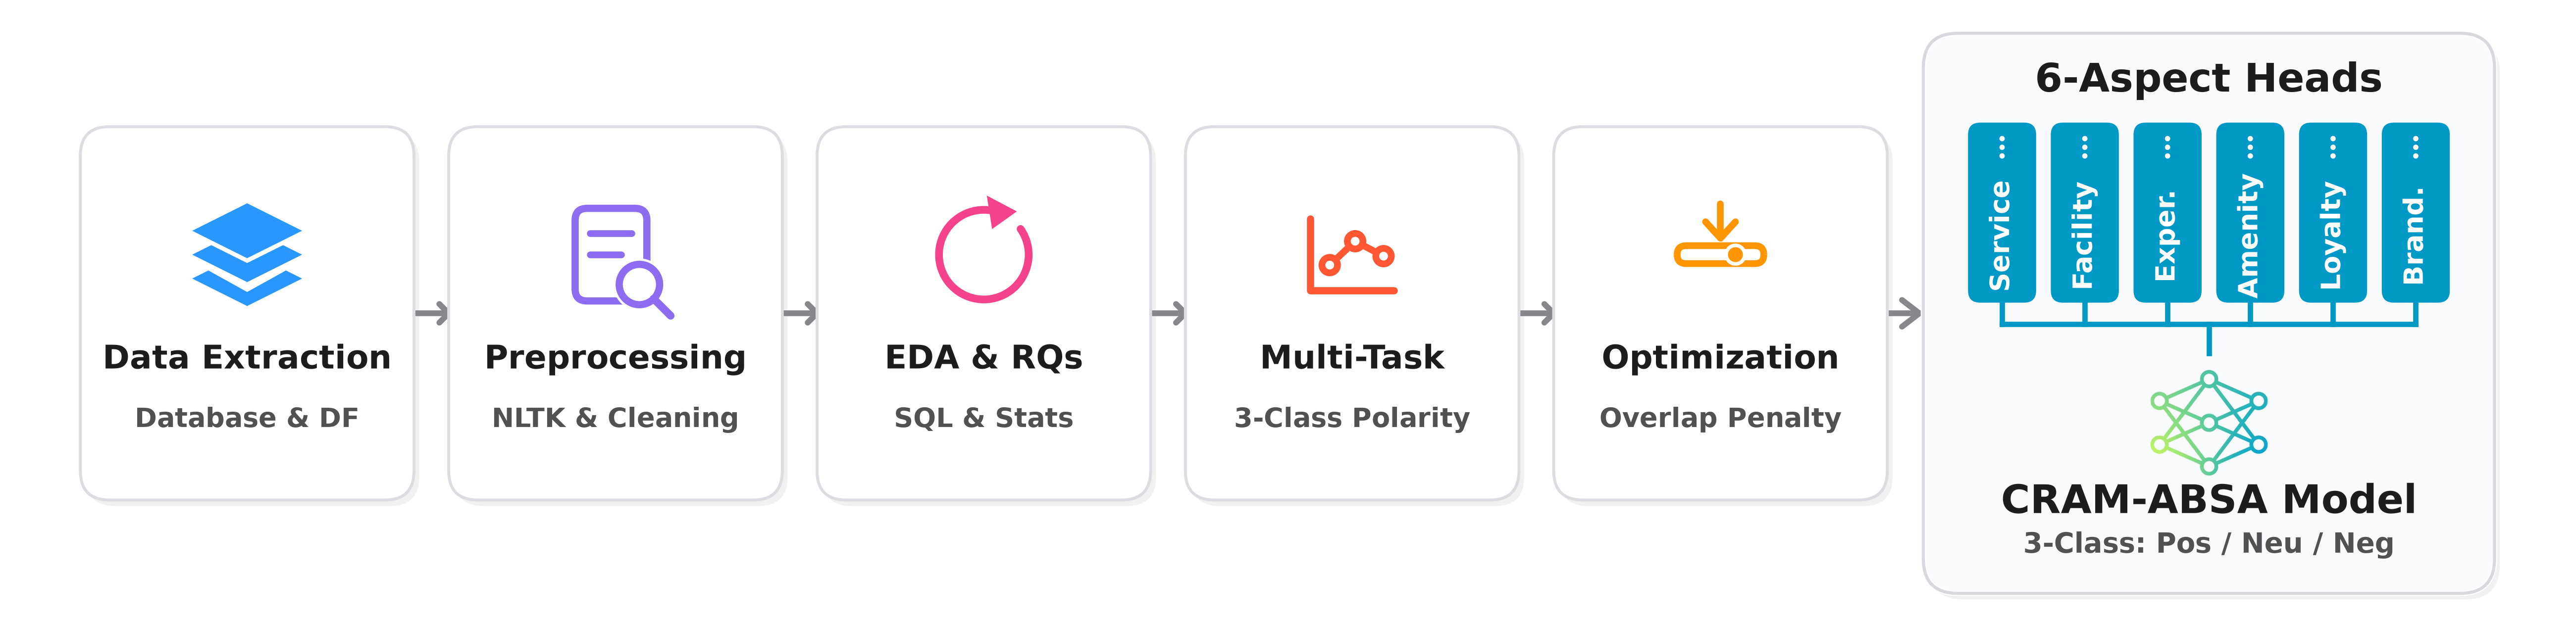
\includegraphics[width=0.98\textwidth]{chart_img/411_research_pipeline.png}
\caption{Overall research pipeline of the proposed study, showing the end-to-end workflow from data extraction and 20-feature engineering to dual-stage CRAM-ABSA modeling and six-metric benchmarking.}
\label{fig:research_pipeline}
\end{figure}

The full research workflow is shown in Fig.~\ref{fig:research_pipeline}. It runs in five main stages: (1) collecting and splitting 9,990 hotel reviews into 80\% training, 10\% validation, and 10\% test sets, (2) exploring the data and building 20 review-level features, (3) Stage 1 negation-aware NLTK text cleaning and embedding-based retrieval (EBR), (4) Stage 2 multi-task BERT modeling with orthogonal rationale masking and CORN ordinal regression, and (5) comparing all models across six evaluation metrics.
\FloatBarrier

\subsection{Stage 1: Negation-Aware Linguistic Processing and Embedding Retrieval}
\label{subsec:stage1_nltk_ebr}
Customer reviews often use short informal phrases and negation words that flip sentiment meaning. Stage 1 prepares clean text signals and finds aspect-relevant sentences before neural modeling:
\begin{itemize}
\item \textbf{Negation-Aware Linguistic Processing (NLTK):} Each review $R$ is normalized to lowercase, contractions (such as \textit{``can't''} or \textit{``n't''}) are expanded, and negation and contrast words (such as \textit{``not''}, \textit{``never''}, \textit{``no''}, \textit{``hardly''}, \textit{``barely''}, \textit{``scarcely''}, \textit{``without''}, and \textit{``but''}) are kept out of stopword removal. When a negation word appears before an opinion word, its polarity is flipped so phrases like \textit{``not clean''} or \textit{``hardly friendly''} are not misread as positive.
\item \textbf{Embedding-Based Retrieval (EBR):} Inspired by RAG \cite{ref23_lewis2020} and dense sentence embeddings \cite{ref24_reimers2019}, we build an aspect exemplar bank from domain keywords and training spans, encoded with \texttt{bert-base-uncased} into prototype vectors $\mathbf{p}_a \in \mathbb{R}^{768}$. For each sentence or token vector $\mathbf{e}_{s_i} \in \mathbb{R}^{768}$, relevance to aspect $a$ is measured by cosine similarity:
\begin{equation}
\text{Sim}(s_i, a) = \frac{\mathbf{e}_{s_i} \cdot \mathbf{p}_a}{\|\mathbf{e}_{s_i}\| \|\mathbf{p}_a\|}
\end{equation}
High-scoring sentences and spans guide the downstream multi-task attention toward real aspect evidence.
\end{itemize}
\FloatBarrier

\subsection{Stage 2: Multi-Task CRAM-ABSA Architecture}
\label{subsec:stage2_cram_absa}
The Stage 2 model combines a shared BERT encoder, residual gating for 20 tabular features, orthogonal rationale masking, and conditional ordinal regression heads (Fig.~\ref{fig:architecture}).

\begin{figure}[ht!]
\centering
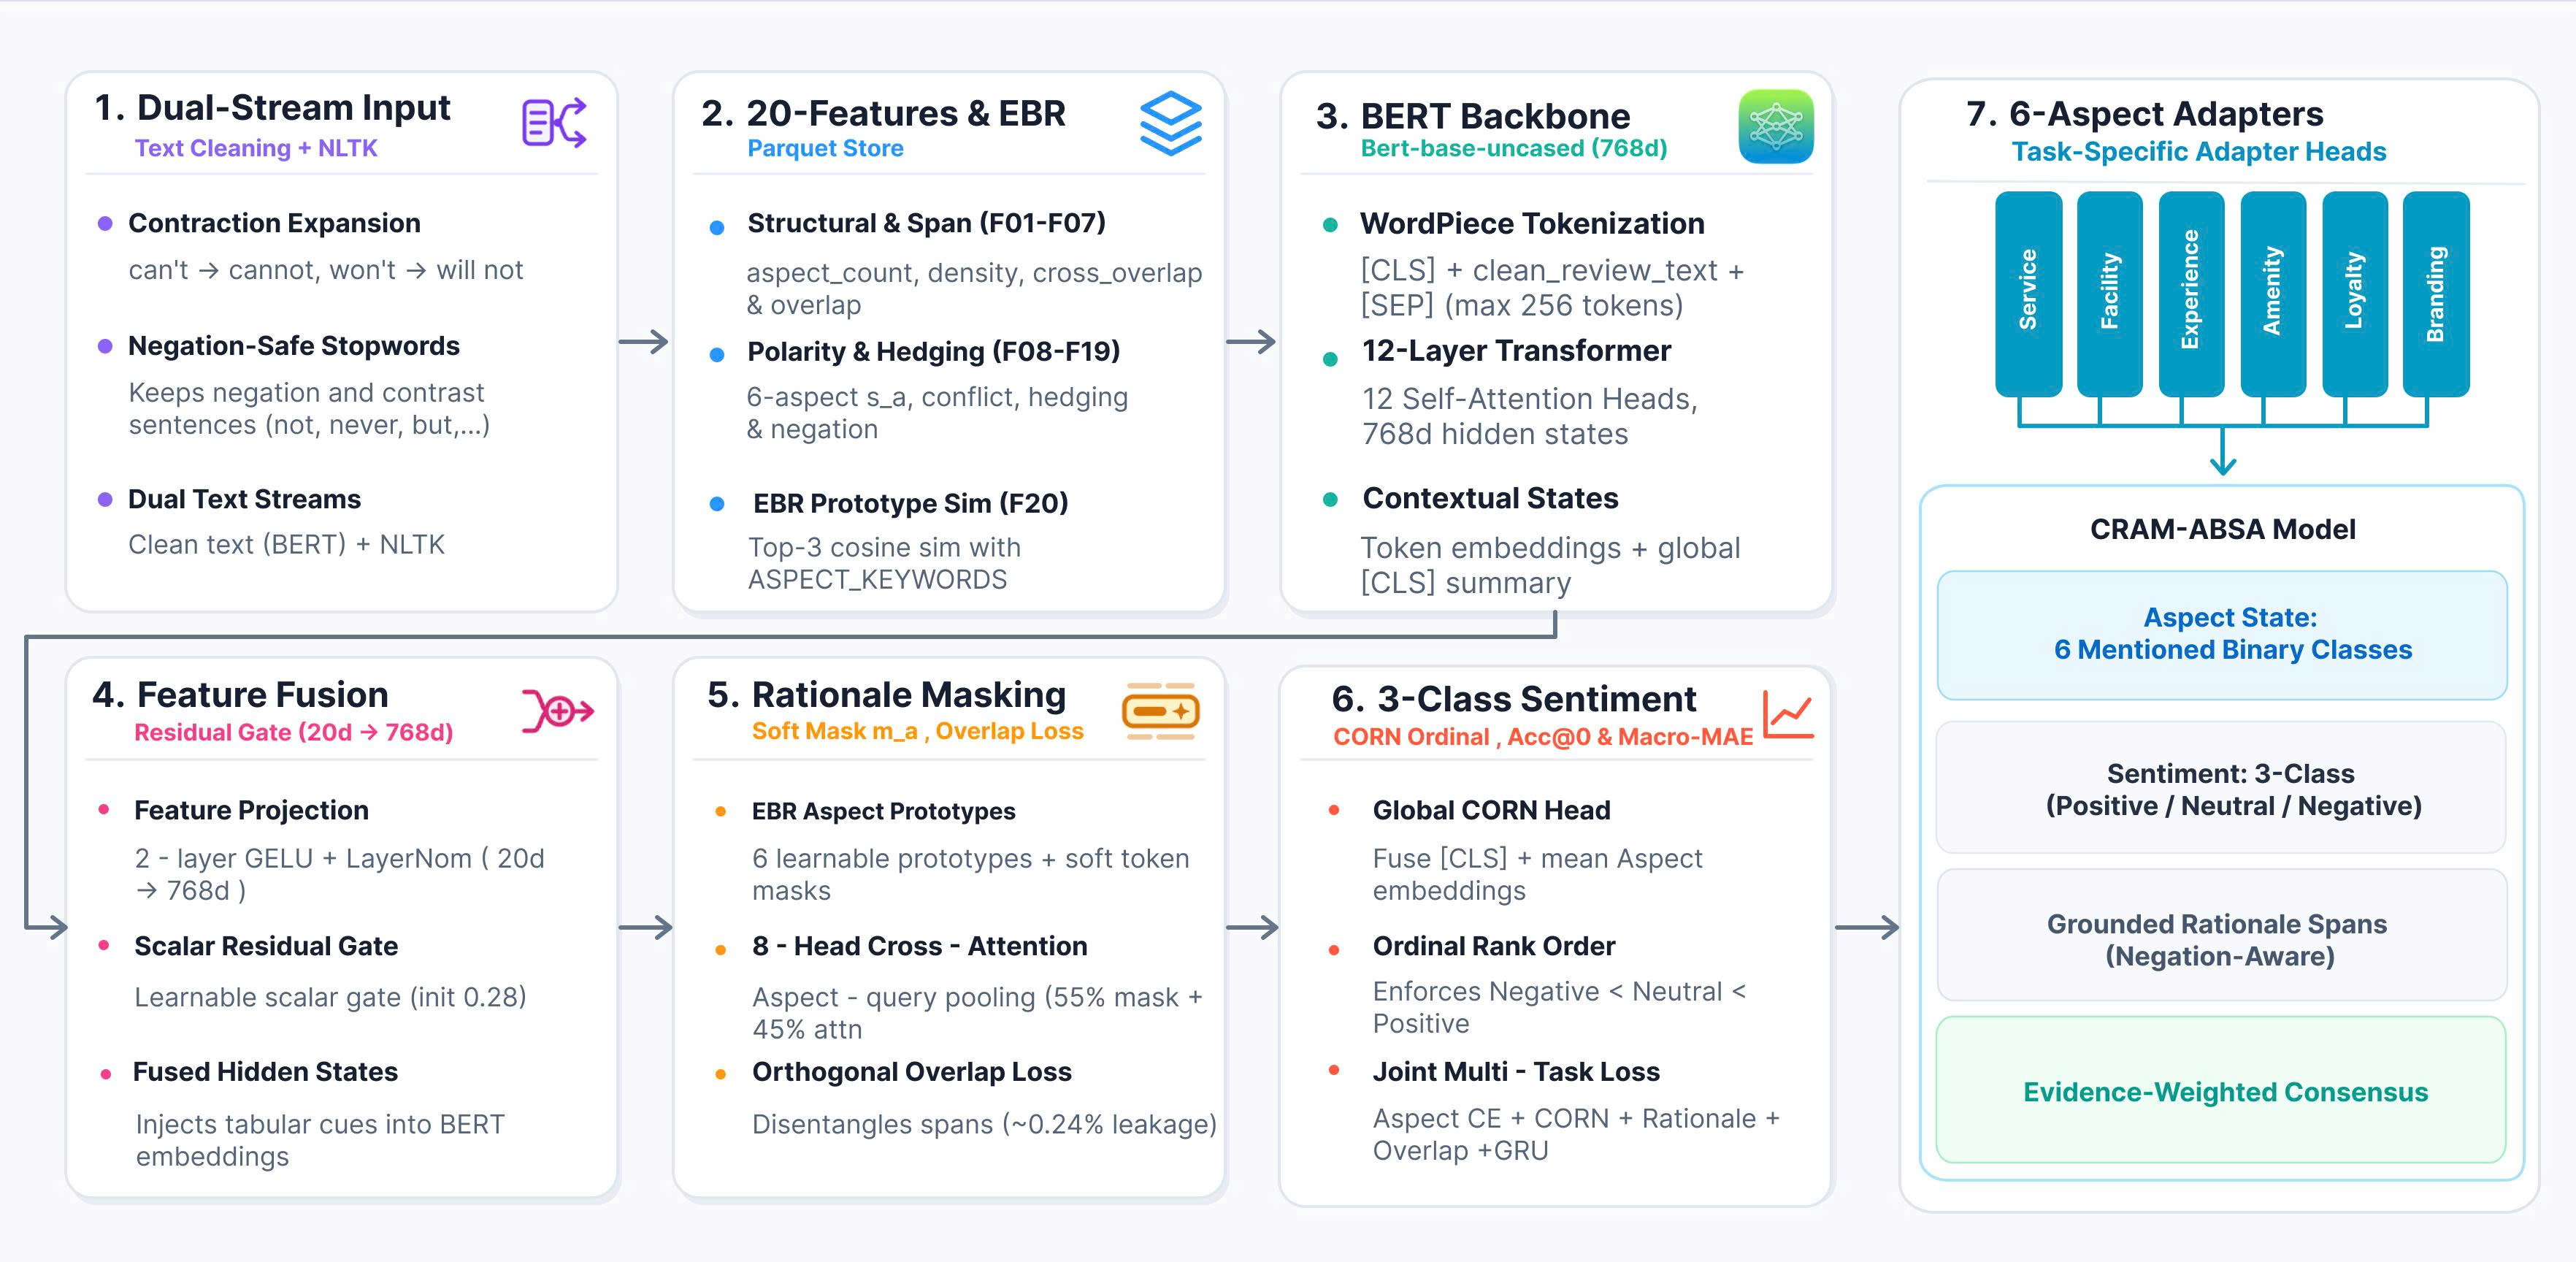
\includegraphics[width=0.86\textwidth]{chart_img/412_model_architecture.png}
\caption{Architecture of the proposed CRAM-ABSA model, combining Stage 1 negation-aware NLTK processing and EBR with Stage 2 BERT encoding, 20-feature residual gating, orthogonal rationale masking, and CORN ordinal regression.}
\label{fig:architecture}
\end{figure}

As shown in Fig.~\ref{fig:architecture}, Stage 2 processes each review through four connected parts:
\begin{itemize}
\item \textbf{Shared Contextual Backbone:} A pretrained \texttt{bert-base-uncased} encoder reads $\text{[CLS]} \, R \, \text{[SEP]}$ and outputs token hidden states $\mathbf{H} \in \mathbb{R}^{n \times 768}$ and a summary vector $\mathbf{h}_{\text{CLS}} \in \mathbb{R}^{768}$.
\item \textbf{Residual Feature Gating:} Twenty engineered tabular features $\mathbf{f} \in \mathbb{R}^{20}$ (covering aspect counts, polarity balance, negation density, and EBR similarity) pass through a two-layer MLP ($20 \rightarrow 256 \rightarrow 768$ with LayerNorm, GELU, and Dropout $0.15$) to produce $\mathbf{f}_{\text{emb}} \in \mathbb{R}^{768}$. This vector is added to the token states through a learnable scalar gate $\alpha \in \mathbb{R}$ (initialized at $\alpha = 0.28$) and directly to the summary vector:
\begin{equation}
\mathbf{H}_{\text{fused}} = \mathbf{H} + \alpha \, \mathbf{f}_{\text{emb}}, \quad \mathbf{h}_{\text{fused}} = \mathbf{h}_{\text{CLS}} + \mathbf{f}_{\text{emb}}
\end{equation}
This residual gate lets tabular signals support the prediction without erasing BERT's language features.
\item \textbf{Orthogonal Rationale Masking and Overlap Loss:} When several aspects appear in one review, standard models often mix up their evidence tokens \cite{ref30_tran2026}. Using EBR aspect prototypes and 8-head cross-attention over $\mathbf{H}_{\text{fused}}$, the model predicts six token rationale masks $\mathbf{m}_a \in (0, 1)^n$ trained with weighted binary cross-entropy ($\mathcal{L}_{\text{rat}}$, positive weight $2.5$). To stop aspects from claiming the same tokens, an overlap loss ($\mathcal{L}_{\text{overlap}}$) combines an off-diagonal Gram-matrix cosine penalty and a token-excess ReLU penalty, reducing cross-aspect leakage to $0.24\%$.
\item \textbf{Aspect, CORN Ordinal, and Joint Loss Heads:} Each aspect has a four-class classifier trained with Cross-Entropy and label smoothing ($0.03$) for $\mathcal{L}_{\text{aspect\_CE}}$. To respect the natural sentiment order ($0 < 1 < 2$), a global CORN head takes $[\mathbf{h}_{\text{fused}}; \bar{\mathbf{z}}] \in \mathbb{R}^{1536}$ (where $\bar{\mathbf{z}}$ is the mean of the six aspect embeddings) and predicts two ordered binary thresholds ($y > 0$ and $y > 1$) for $\mathcal{L}_{\text{CORN}}$. A lightweight GRU commentary head ($\mathcal{L}_{\text{com}}$) also supports evidence decoding. The full multi-task loss is:
\begin{equation}
\mathcal{L}_{\text{total}} = \mathcal{L}_{\text{aspect\_CE}} + \beta_{\text{CORN}} \mathcal{L}_{\text{CORN}} + \beta_{\text{rat}} \mathcal{L}_{\text{rat}} + \beta_{\text{overlap}} \mathcal{L}_{\text{overlap}} + \beta_{\text{com}} \mathcal{L}_{\text{com}}
\end{equation}
with weights set to $\beta_{\text{CORN}} = 0.20$, $\beta_{\text{rat}} = 0.25$, $\beta_{\text{overlap}} = 0.35$, and $\beta_{\text{com}} = 0.05$.
\end{itemize}
\FloatBarrier

%========================================================
% 4. EXPERIMENTS
%========================================================
\section{Experimental Evaluation}
\label{sec:experimental_evaluation}

\subsection{Dataset and 20-Feature Engineering}
\label{subsec:dataset_eda_features}
We evaluate CRAM-ABSA on a dataset of 9,990 hotel reviews from major online booking platforms \cite{ref10_nguyen2023,ref25_le2026}. We split the data using an 80/10/10 ratio: 7,992 reviews for training, 999 for validation, and an independent test set of \textbf{999 reviews}. Each review is labeled across six aspects (\textit{Service}, \textit{Facility}, \textit{Experience}, \textit{Amenity}, \textit{Loyalty}, and \textit{Branding}) with four states per aspect (\textit{Not Mentioned, Negative, Neutral, Positive}).

\begin{figure}[ht!]
\centering
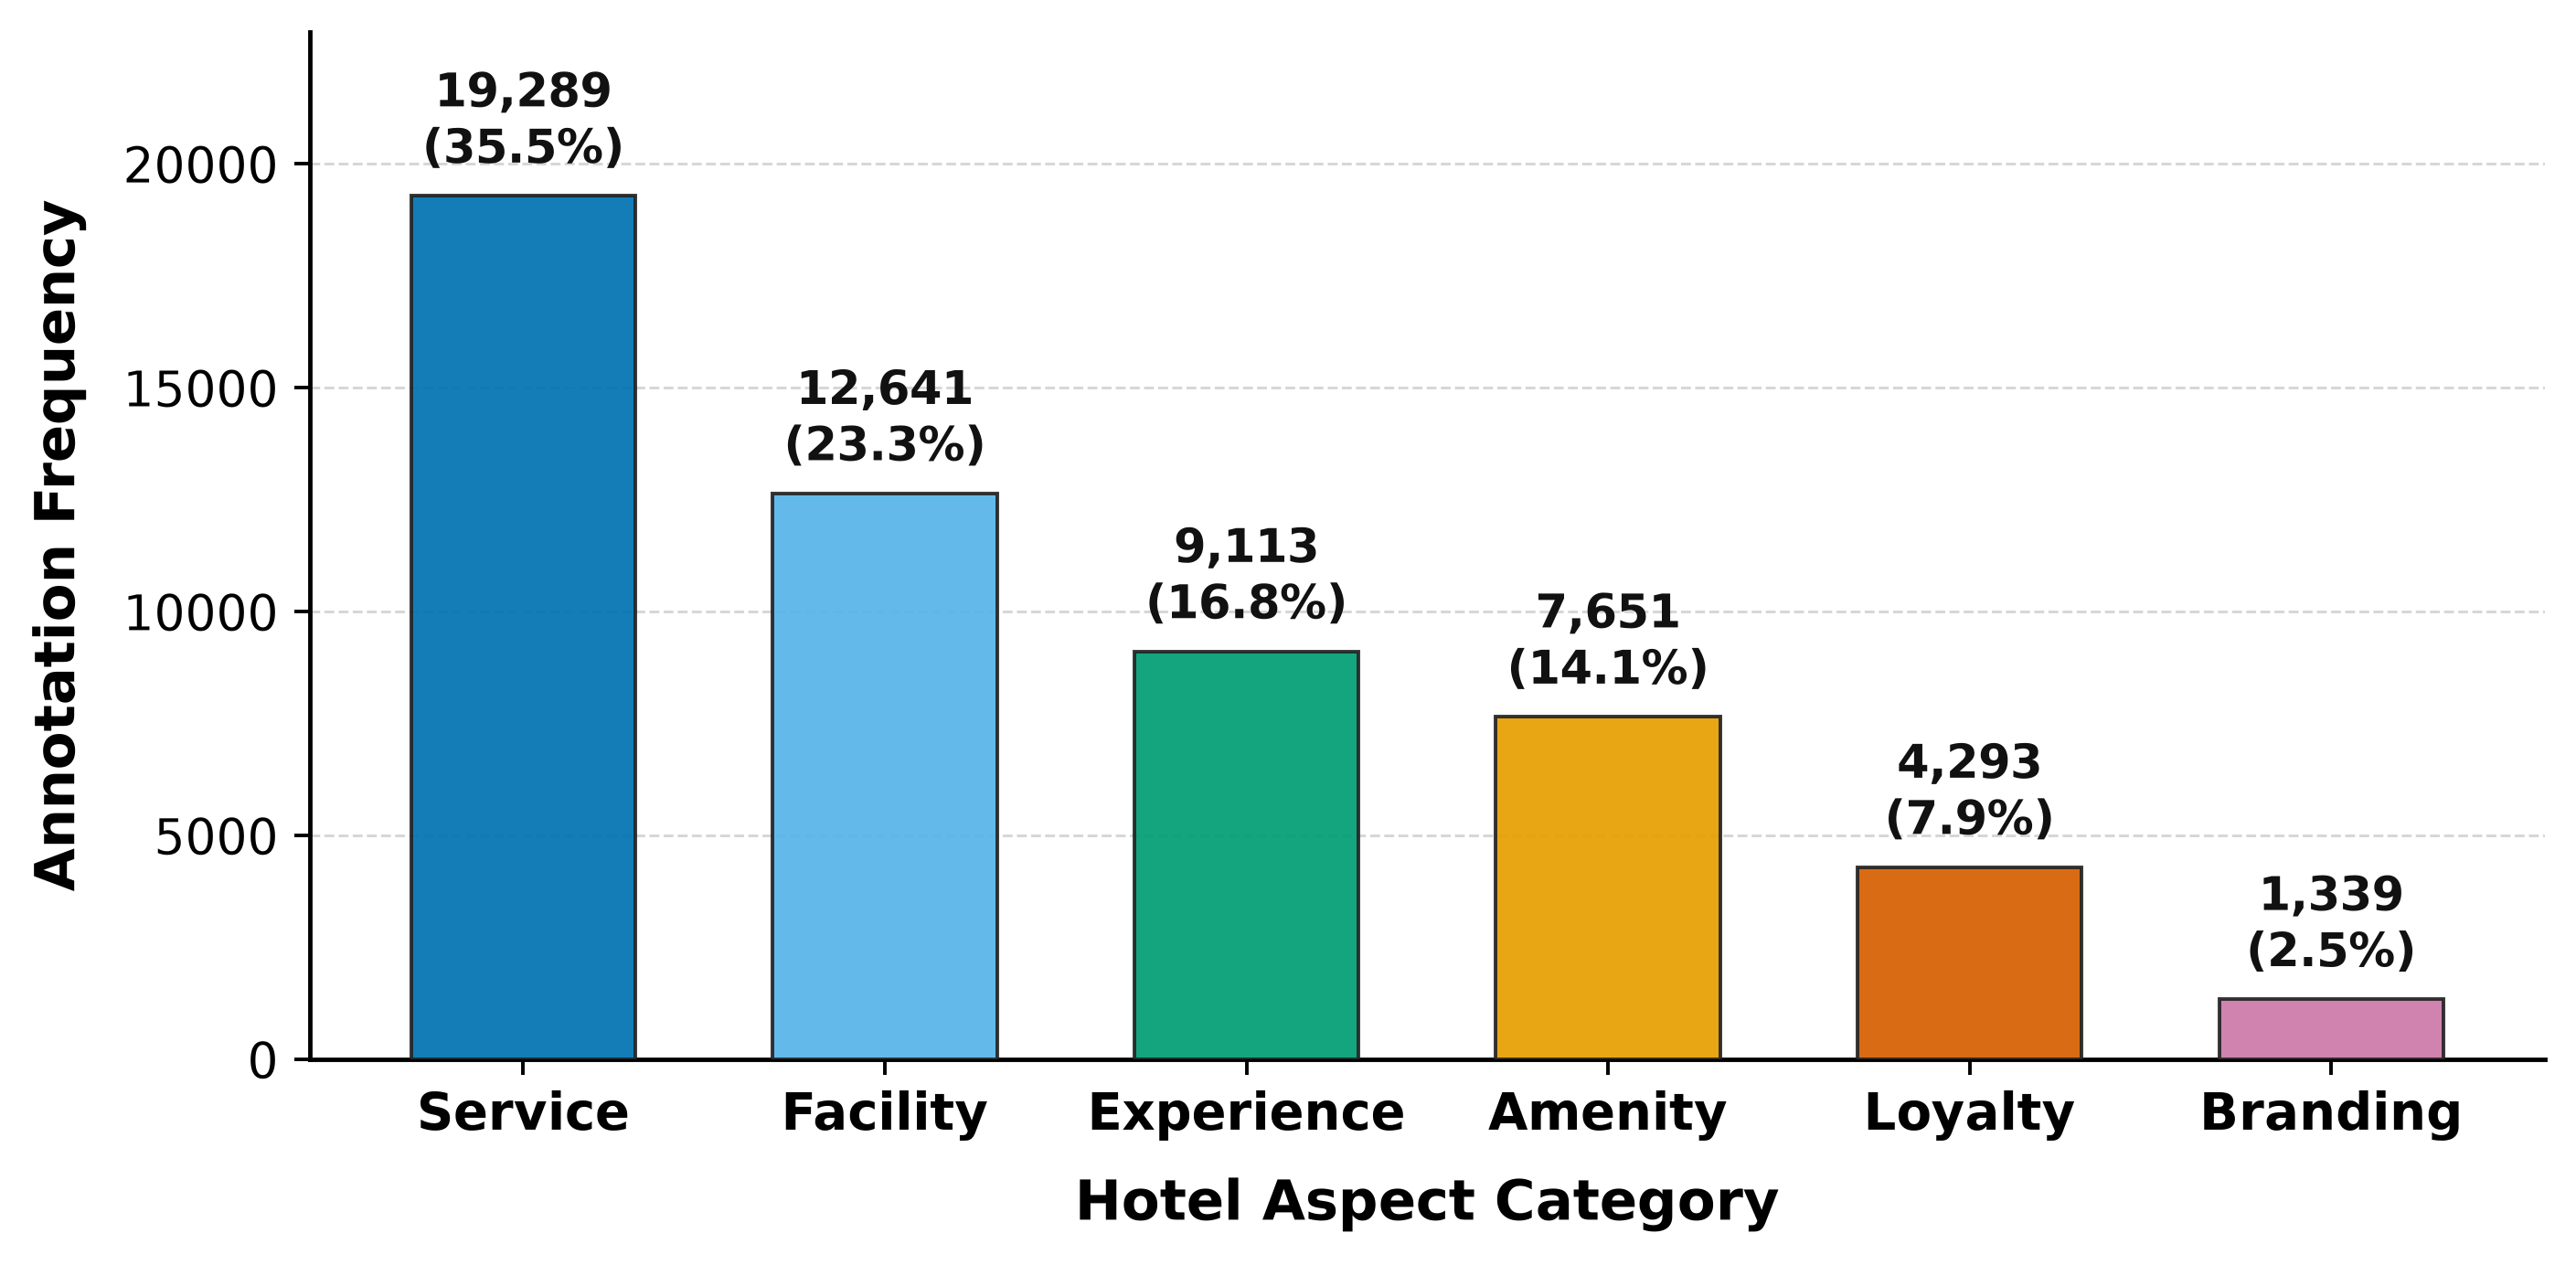
\includegraphics[width=0.78\textwidth]{chart_img/43_aspect_frequency_distribution.png}
\caption{Aspect frequency distribution across the 9,990 review corpus.}
\label{fig:aspect_freq}
\end{figure}

\begin{figure}[ht!]
\centering
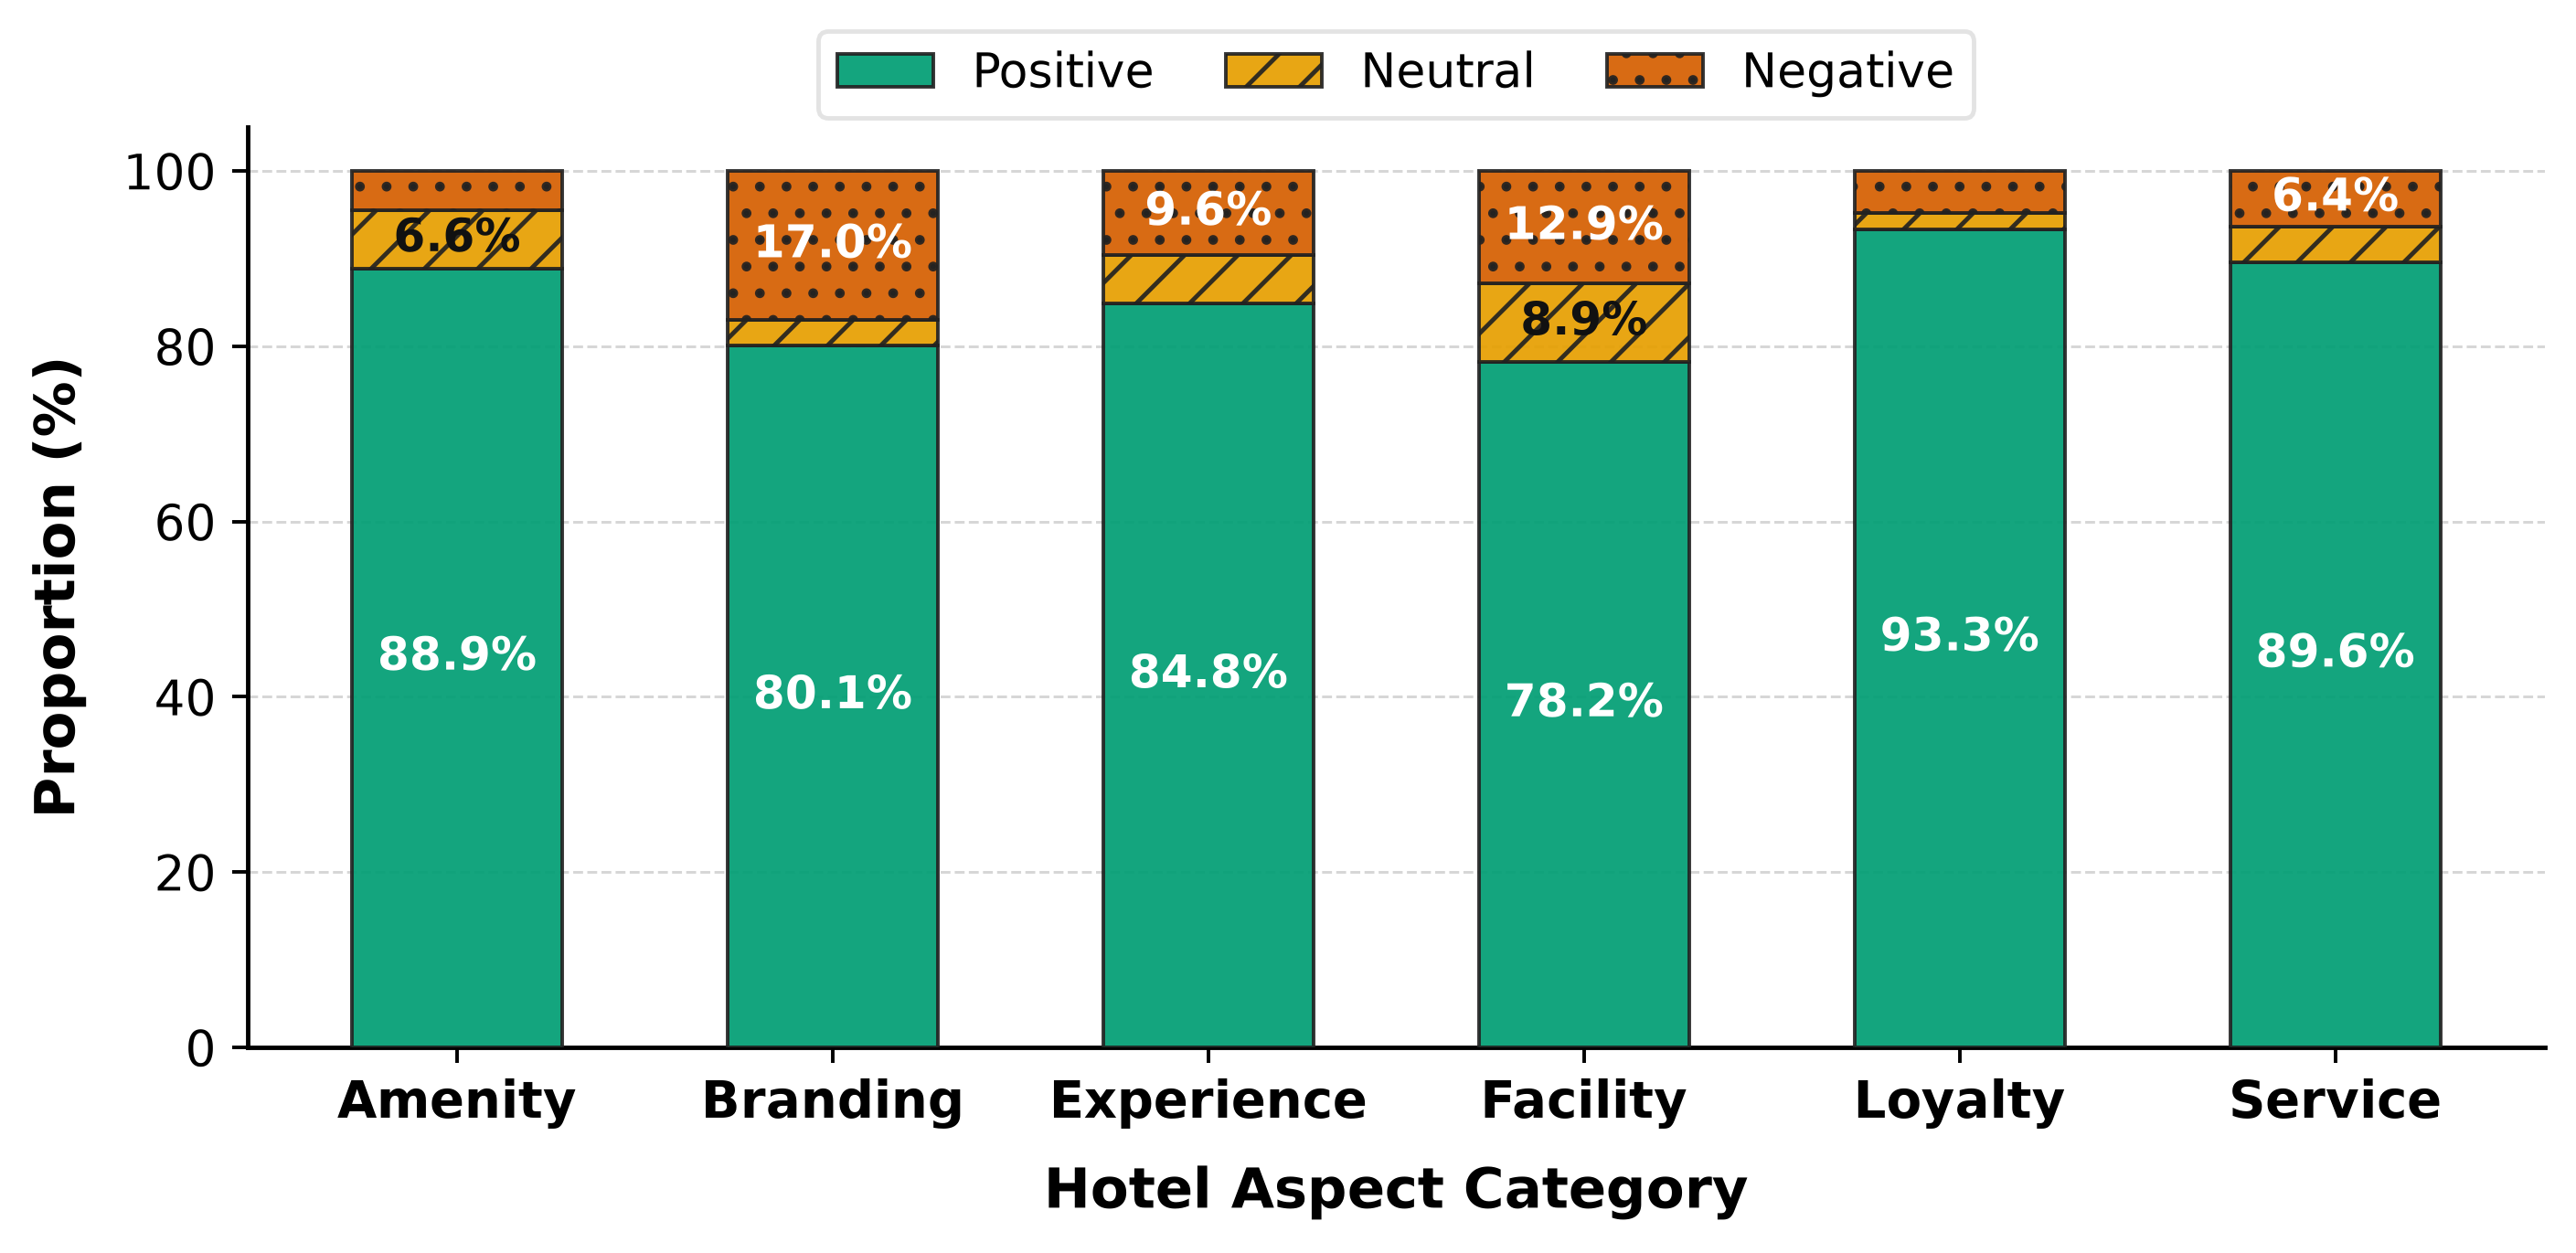
\includegraphics[width=0.78\textwidth]{chart_img/44_aspect_sentiment_breakdown.png}
\caption{Sentiment breakdown across the six evaluated hotel aspects.}
\label{fig:sentiment_breakdown}
\end{figure}

As shown in Fig.~\ref{fig:aspect_freq}, the dataset is strongly imbalanced: \textit{Service} and \textit{Facility} appear very often, while \textit{Loyalty} and \textit{Branding} are rare. Also, Fig.~\ref{fig:sentiment_breakdown} shows that positive sentiments are much more common than negative or neutral ones across all six aspects.

To handle this imbalance, we build 20 tabular features in four groups: (1)~\textit{Aspect Structure} (Feats 01--03, 14: mention count, main aspect, aspect share, text coverage); (2)~\textit{Sentiment Polarity} (Feats 04, 08--13, 17: net sentiment, conflict flag, six aspect sentiment scores, lexical polarity strength); (3)~\textit{Text Evidence} (Feats 05--07, 15--16: evidence density, average token length, overlap flag, hedging density, consensus score); and (4)~\textit{Linguistic and EBR} (Feats 18--20: clean token ratio, negation density, Top-3 EBR centroid similarities).
\FloatBarrier

\subsection{Baseline Models and Implementation Details}
\label{subsec:baselines_implementation}
We compare CRAM-ABSA against three published baseline models:
\begin{enumerate}
    \item \textbf{BERT-Base (Bimaputra and Sutoyo, 2023 \cite{ref01_bimaputra2023}):} A standard BERT-base model fine-tuned on hotel reviews with a separate classifier head for each aspect.
    \item \textbf{BM25-CNN (Namee et al., 2023 \cite{ref04_namee2023}):} A hybrid model combining BM25 keyword matching, TF-IGM, Support Vector Machines (SVM), and a Multi-Region CNN.
    \item \textbf{WSD-BiLSTM-GCN (Nadeem et al., 2025 \cite{ref09_nadeem2025}):} A model that uses Word Sense Disambiguation (WSD) and Graph Convolutional Networks (GCN) over syntax trees.
\end{enumerate}

All models are trained and tested on the exact same 999-review test split. Deep models use the AdamW optimizer with a learning rate of $2 \times 10^{-5}$, 10\% linear warmup, and cosine decay. The batch size is 32, dropout is 0.1, and training runs for up to 10 epochs with early stopping on validation loss.

\subsection{Evaluation Metrics}
\label{subsec:evaluation_metrics}
We evaluate all models using six metrics on the 999-review test set: (1)~\textbf{Acc@0 (\%) $\uparrow$:} exact-match sentiment accuracy (zero rating error); (2)~\textbf{6-Aspect Macro-F1 (\%) $\uparrow$:} average Macro-F1 across all six aspects and four states; (3)~\textbf{Macro-MAE $\downarrow$:} average ordinal distance error across sentiment classes (penalizing opposite-polarity errors by 2); (4)~\textbf{Rationale F1 (\%) $\uparrow$:} token-level overlap F1 against human-labeled evidence spans; (5)~\textbf{Leakage (\%) $\downarrow$:} share of tokens assigned to two or more aspects; and (6)~\textbf{Test Loss $\downarrow$:} total multi-task loss on the test set.

\FloatBarrier
\subsection{Overall Quantitative Benchmark Results}
\label{subsec:overall_results}
Table~\ref{tab:overall_benchmark} and Fig.~\ref{fig:benchmark_comparison} show the results of CRAM-ABSA and the three baseline models on the 999-review test set.

\begin{table}[ht!]
\caption{Benchmark evaluation results on the independent test split (999 samples). Arrows indicate whether higher ($\uparrow$) or lower ($\downarrow$) values are preferred. Best results across each column are shown in \textbf{bold}.}\label{tab:overall_benchmark}
\small
\setlength{\tabcolsep}{3pt}
\begin{tabular*}{\textwidth}{@{\extracolsep{\fill}}lcccccr@{}}
\toprule
\textbf{Model} & \textbf{Test} & \textbf{Acc@0} & \textbf{Macro-F1} & \textbf{Macro-} & \textbf{Rat-F1} & \textbf{Leak} \\
\textbf{Architecture} & \textbf{Loss} $\downarrow$ & \textbf{(\%)} $\uparrow$ & \textbf{(\%)} $\uparrow$ & \textbf{MAE} $\downarrow$ & \textbf{(\%)} $\uparrow$ & \textbf{(\%)} $\downarrow$ \\
\midrule
\textbf{CRAM-ABSA (Ours)} & \textbf{0.2552} & 92.39 & \textbf{72.55} & \textbf{0.3520} & \textbf{70.84} & 0.24 \\
BERT-Base \cite{ref01_bimaputra2023} & 0.5143 & 92.29 & 52.55 & 0.4823 & 50.66 & \textbf{0.02} \\
BM25-CNN \cite{ref04_namee2023} & 0.6032 & 91.69 & 44.22 & 0.6743 & 32.65 & 54.47 \\
WSD-BiLSTM-GCN \cite{ref09_nadeem2025} & 0.5227 & \textbf{92.59} & 52.12 & 0.4756 & 9.77 & 0.22 \\
\botrule
\end{tabular*}
\end{table}

\begin{figure}[ht!]
\centering
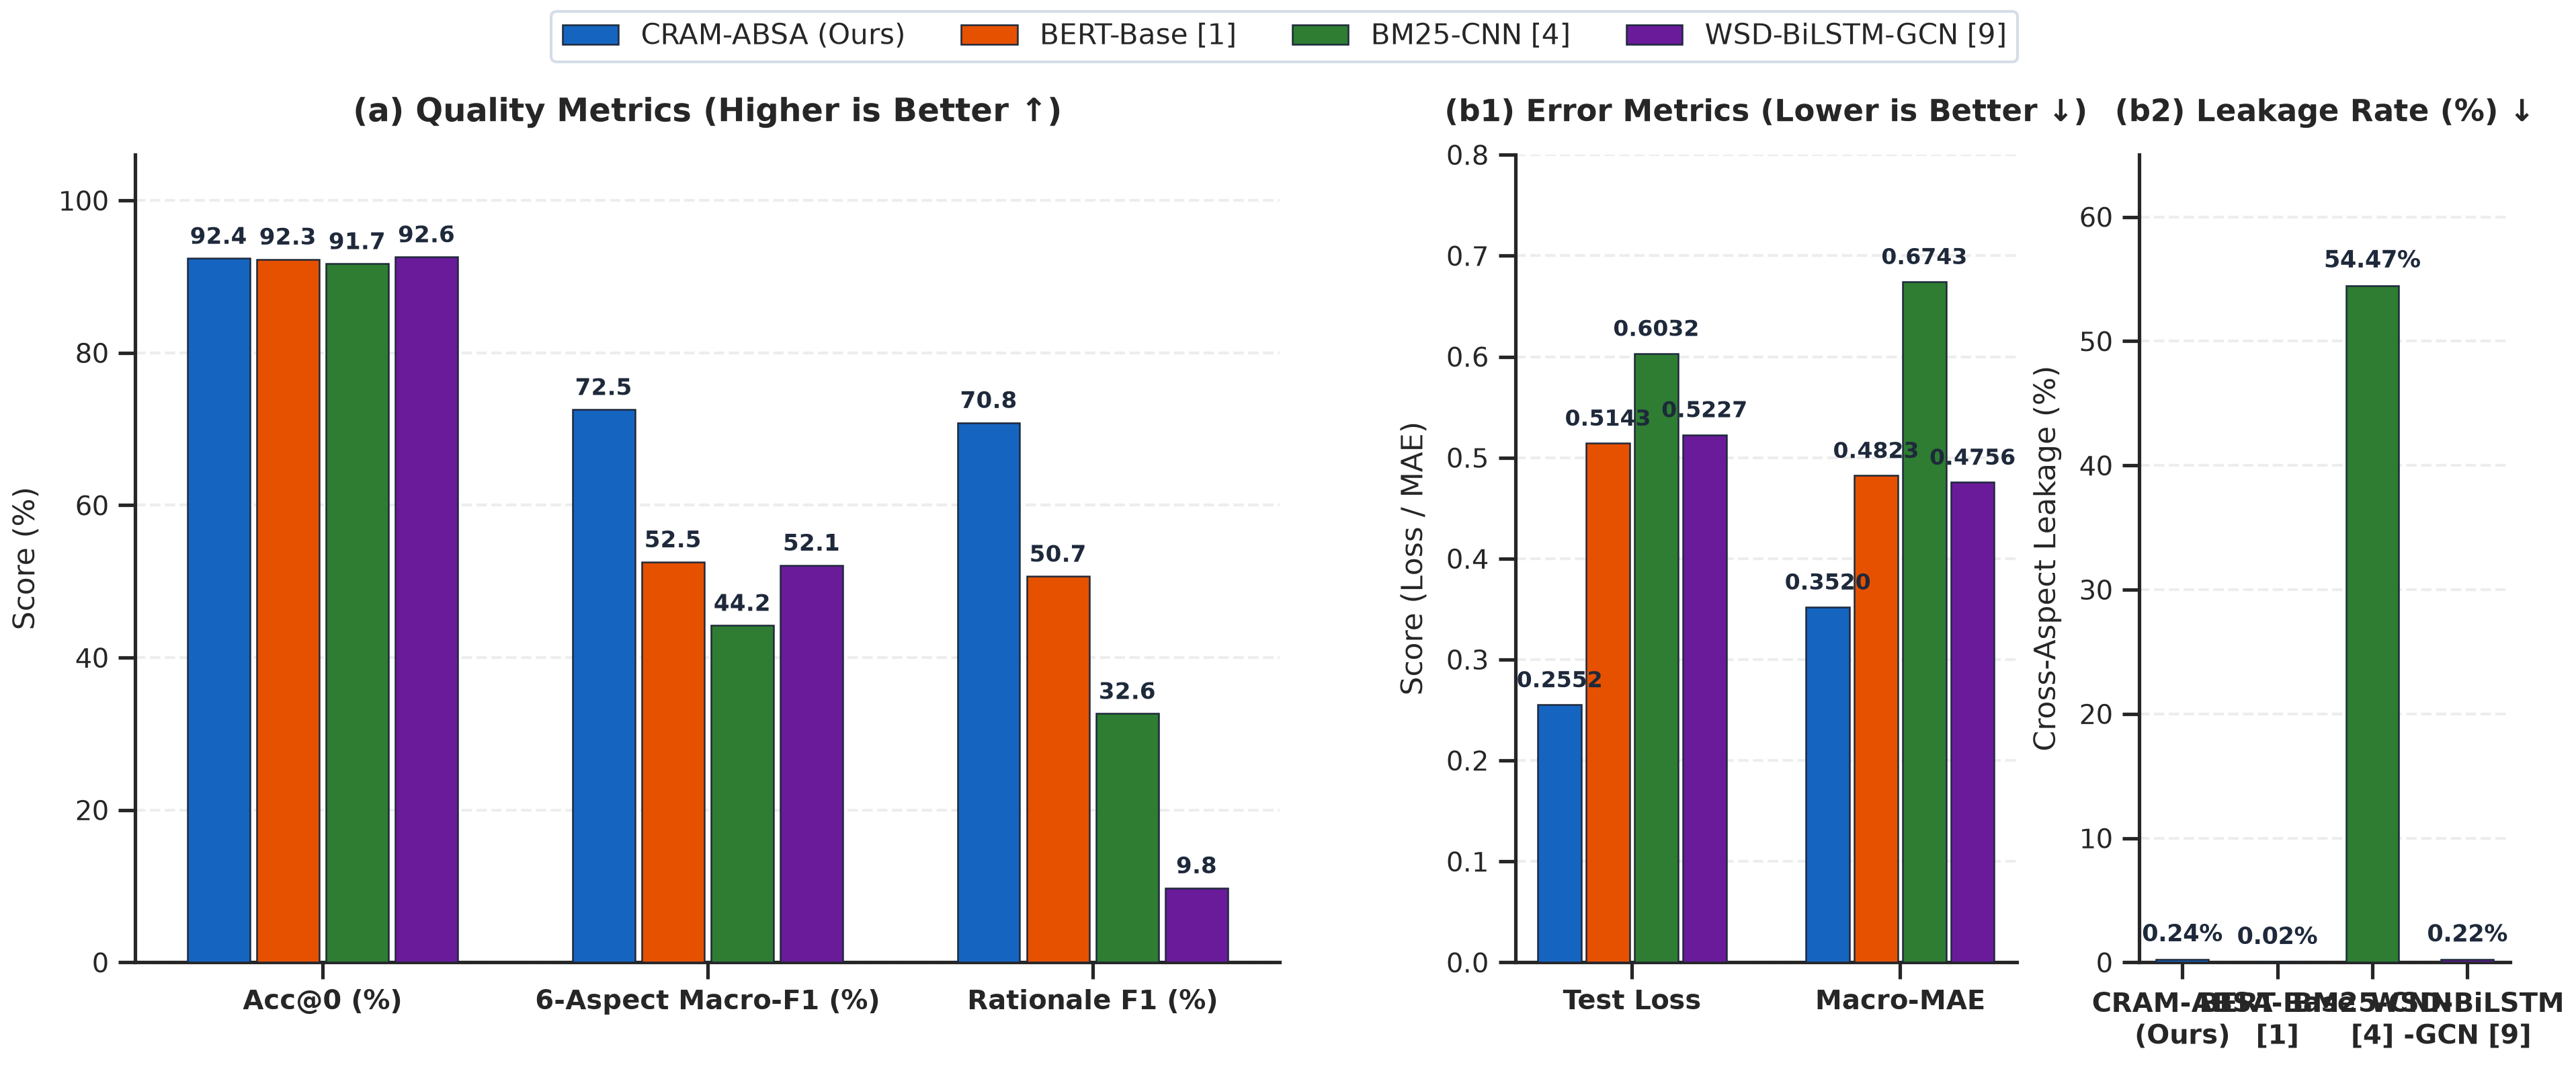
\includegraphics[width=0.80\textwidth]{chart_img/413_benchmark_comparison.png}
\caption{Quality metric comparison on the 999-sample independent test split across the four evaluated models, covering Acc@0, 6-Aspect Macro-F1, and Rationale F1 (higher $\uparrow$ is better).}
\label{fig:benchmark_comparison}
\end{figure}

Overall, CRAM-ABSA leads in 4 out of 6 metrics:
(1)~\textit{Lowest Test Loss (0.2552):} more than 50\% lower than the baselines (0.5143--0.6032);
(2)~\textit{Highest 6-Aspect Macro-F1 (72.55\%):} +20.00 percentage points above BERT-Base (52.55\%), +20.43 above WSD-BiLSTM-GCN (52.12\%), and +28.33 above BM25-CNN (44.22\%);
(3)~\textit{Lowest Macro-MAE (0.3520):} clearly below WSD-BiLSTM-GCN (0.4756), BERT-Base (0.4823), and BM25-CNN (0.6743);
(4)~\textit{Highest Rationale F1 (70.84\%):} well ahead of BERT-Base (50.66\%), BM25-CNN (32.65\%), and WSD-BiLSTM-GCN (9.77\%); and
(5)~\textit{Low Leakage (0.24\%) with High Acc@0 (92.39\%):} close to the top Acc@0 of WSD-BiLSTM-GCN (92.59\%) while avoiding the 54.47\% leakage of BM25-CNN (BERT-Base has 0.02\% leakage).
\FloatBarrier

\subsection{Metric Interpretation Across Research Questions (RQ1--RQ3)}
\label{subsec:rq_interpretation}
We now explain what these benchmark numbers mean for our three Research Questions:

\begin{figure}[ht!]
\centering
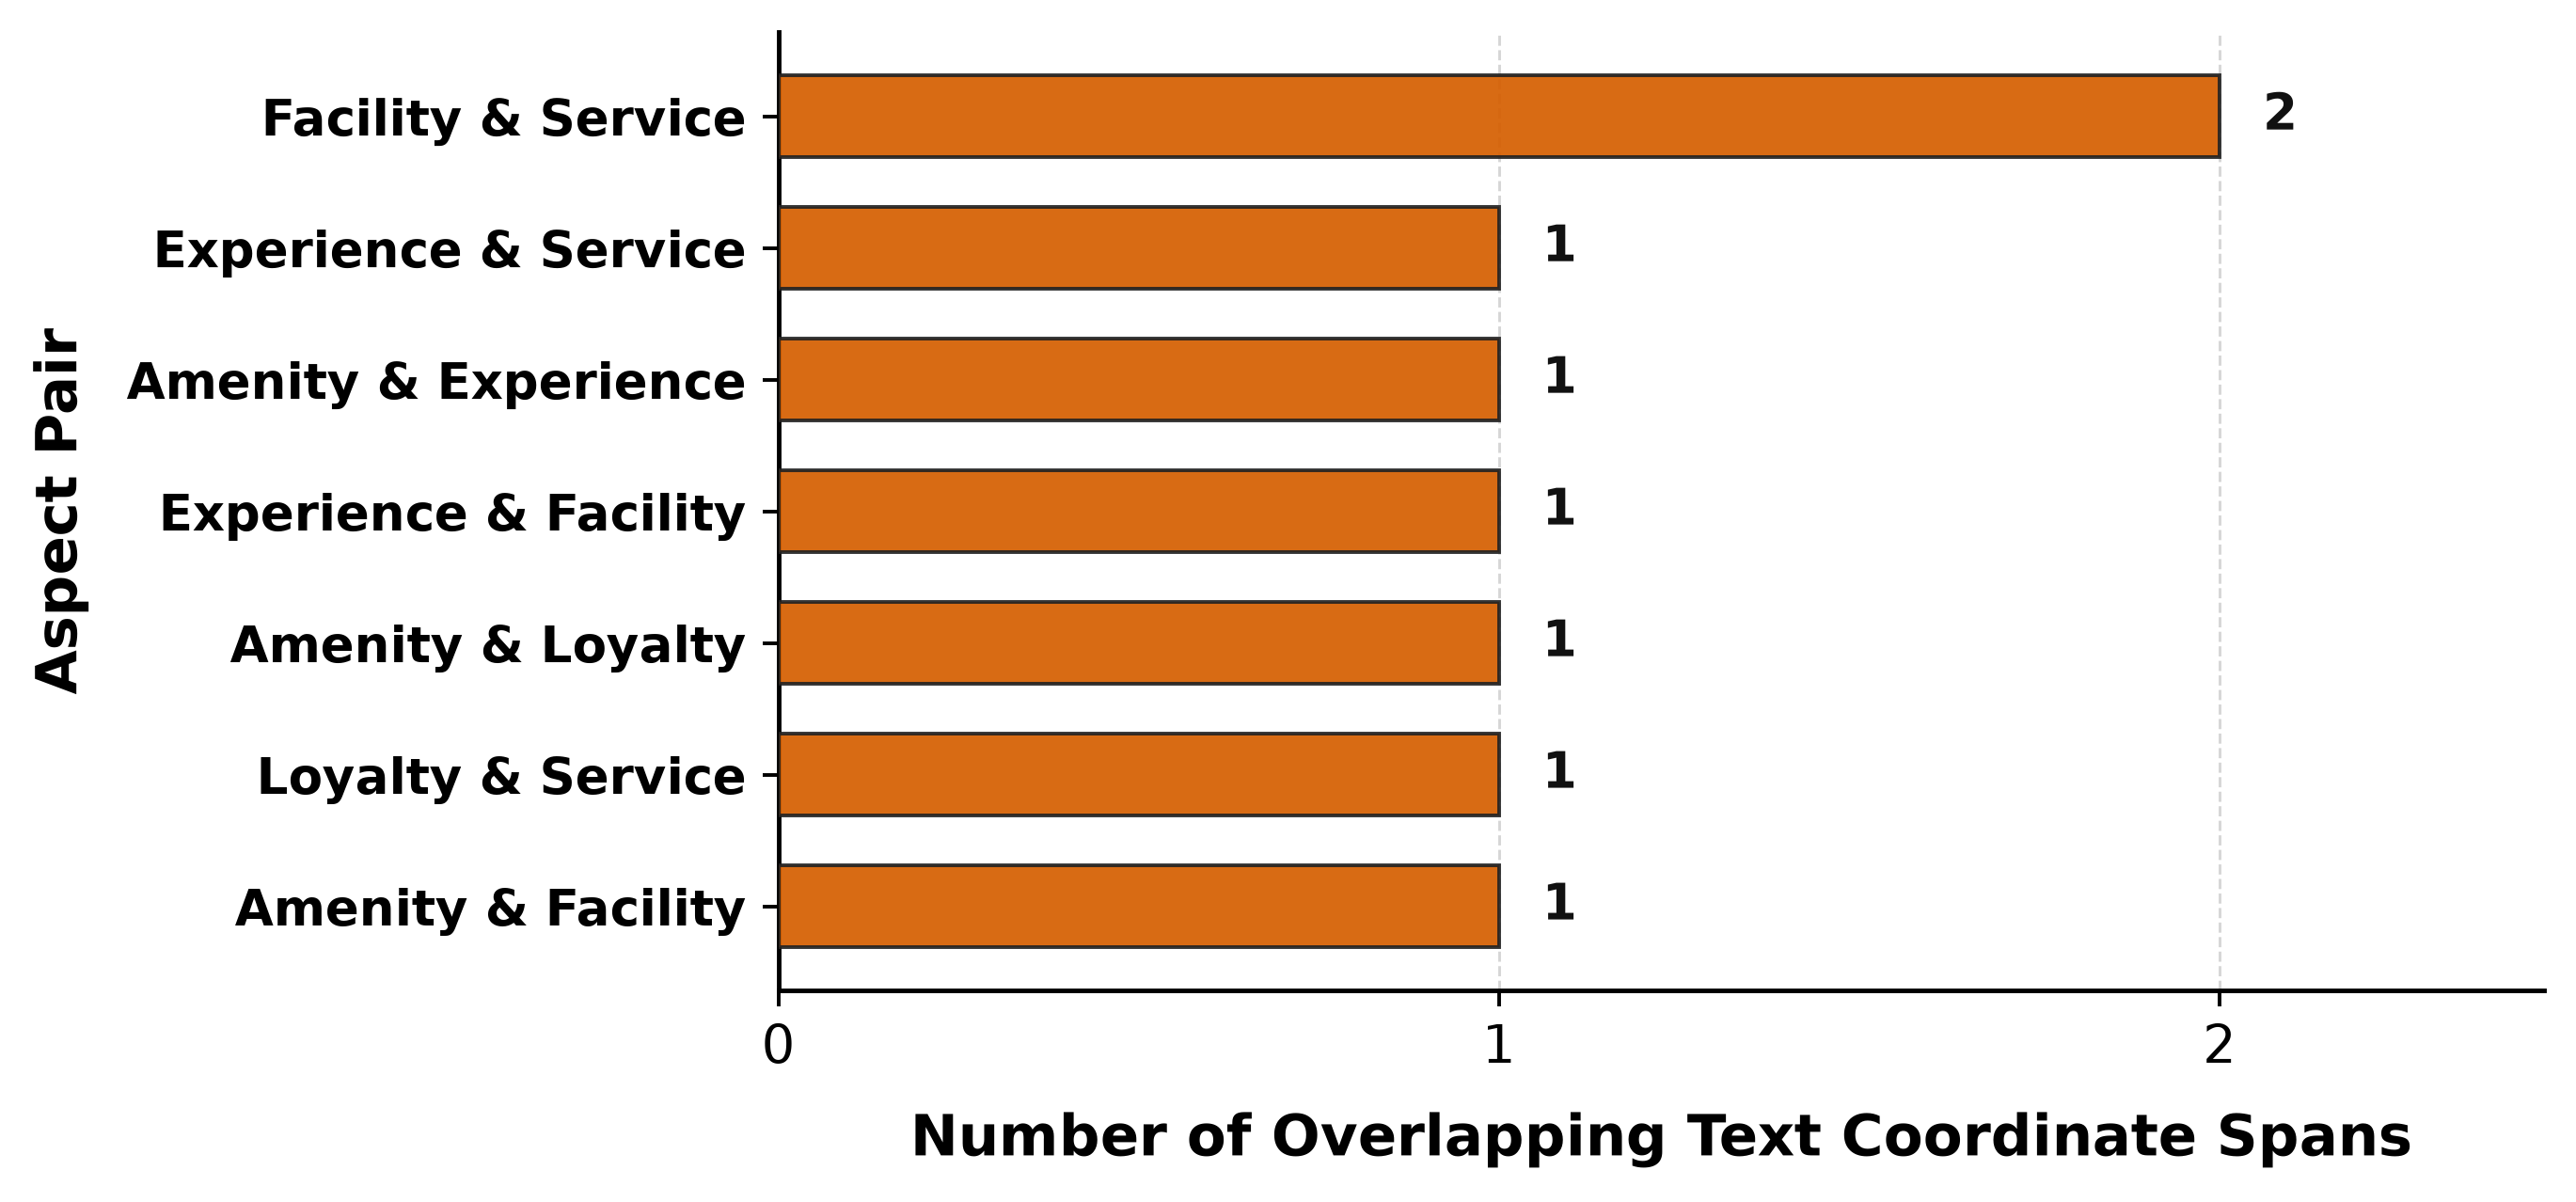
\includegraphics[width=0.78\textwidth]{chart_img/49_cross_aspect_span_overlap.png}
\caption{Counts of overlapping text coordinate spans across hotel aspect pairs.}
\label{fig:span_overlap}
\end{figure}

\begin{figure}[ht!]
\centering
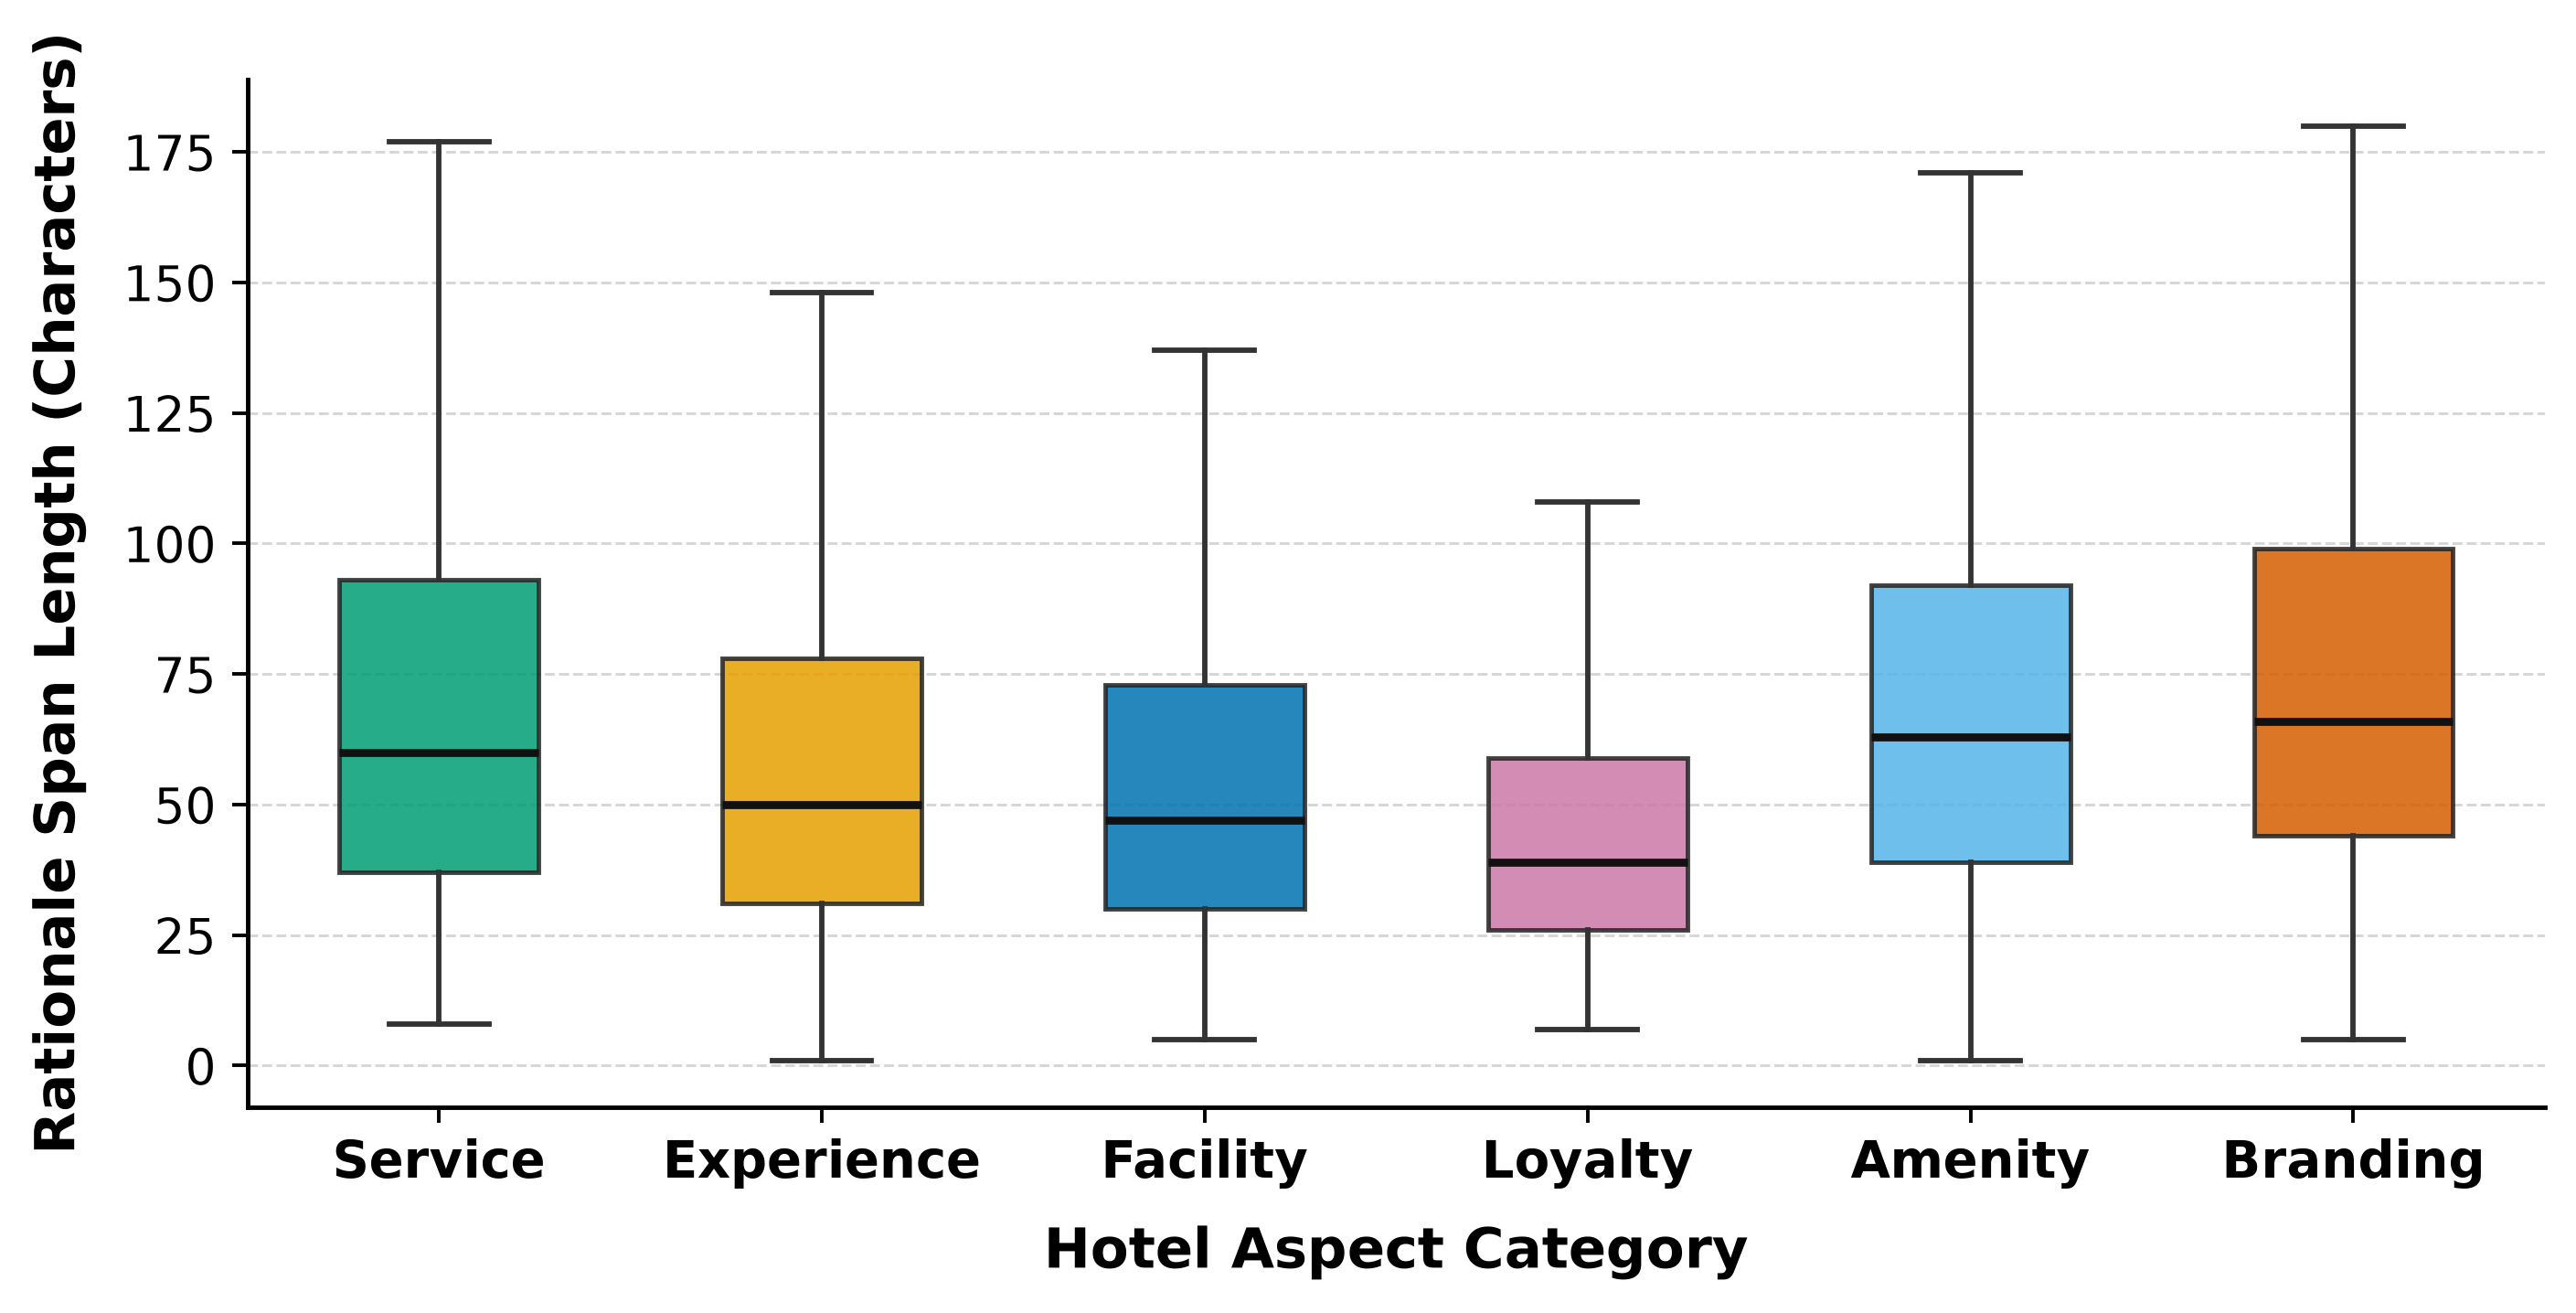
\includegraphics[width=0.78\textwidth]{chart_img/45_rationale_length_by_aspect.png}
\caption{Distribution of rationale span lengths (in characters) across the six aspects.}
\label{fig:rationale_length}
\end{figure}

\begin{itemize}
    \item \textbf{RQ1 (Multi-Aspect Sentiment Classification):} Baseline models reach high Acc@0 (91.69--92.59\%) mostly because they predict common \textit{Not Mentioned} and positive labels (Fig.~\ref{fig:aspect_freq} and Fig.~\ref{fig:sentiment_breakdown}). However, their Macro-F1 drops to 44.22--52.55\% on rare aspects (\textit{Loyalty}, \textit{Branding}) and negative or neutral cases. By combining text embeddings with the 20 tabular features via residual gating, CRAM-ABSA lifts Macro-F1 to 72.55\% while keeping Acc@0 at 92.39\%.
    \item \textbf{RQ2 (Leakage Control and Ordinal Consistency):} CRAM-ABSA lowers Macro-MAE to 0.3520 (vs.\ 0.4756--0.6743) because CORN ordinal regression reduces large opposite-polarity errors. Meanwhile, Fig.~\ref{fig:span_overlap} shows that ground-truth aspect spans rarely overlap (only 8 cases total). BM25-CNN's keyword rules cause 54.47\% leakage, and BERT-Base's 0.02\% leakage comes from separate heads with lower Rationale F1 (50.66\%). CRAM-ABSA's orthogonal masking keeps leakage at 0.24\% while reaching 70.84\% Rationale F1.
    \item \textbf{RQ3 (Evidence Extraction):} As shown in Fig.~\ref{fig:rationale_length}, human-labeled evidence spans are short, with median lengths of about 39 to 66 characters. Baselines struggle to find these spans (9.77--50.66\% Rationale F1) because they lack explicit span alignment or fail on negation. Stage~1 negation-aware filtering and EBR retrieval help CRAM-ABSA reach 70.84\% Rationale F1 and extract accurate, grounded evidence.
\end{itemize}
\FloatBarrier

%========================================================
% 5. DISCUSSION AND CONCLUSION
%========================================================
\section{Discussion and Conclusion}
\label{sec:discussion_conclusion}

\subsection{Practical and Managerial Implications}
\label{subsec:discussion_implications}
Our results offer useful lessons for both hospitality research and hotel management. From a research view, CRAM-ABSA solves key trade-offs between multi-aspect coverage, cross-aspect leakage, and ordinal rating accuracy. Linking neural embeddings to explicit text evidence also makes model predictions easier to explain \cite{ref16_shin2024}. From a business view, tracking all six aspects (\textit{Service, Facility, Experience, Amenity, Loyalty, Branding}) gives hotel managers a clearer picture than a single overall score. Managers can use penalty-reward analysis \cite{ref13_zhang2022} to find the main causes of guest complaints, and guest-relation teams can use extracted evidence spans to respond quickly and fix service problems \cite{ref15_pang2025}.

\subsection{Conclusion, Limitations and Future Work}
\label{subsec:conclusion_future_work}
This paper presented \textbf{CRAM-ABSA}, a multi-task model for six-aspect hotel review assessment and evidence extraction. By combining negation-aware NLTK filtering and dense EBR with orthogonal masking, 20-feature residual gating, and conditional ordinal regression, CRAM-ABSA overcomes key limits of existing baselines \cite{ref01_bimaputra2023,ref04_namee2023,ref09_nadeem2025}. On the 999-sample test split, CRAM-ABSA leads in 4 of 6 metrics: it reaches the lowest Test Loss (0.2552), highest 6-Aspect Macro-F1 (72.55\%, a +20\% gain), lowest Macro-MAE (0.3520), and highest Rationale F1 (70.84\%), while keeping leakage low at 0.24\% and Acc@0 high at 92.39\%. One limitation is that our evaluation uses a single data split. In future work, we plan to run multi-fold cross-validation, test parameter ablation grids, and adapt the model to multiple languages across Southeast Asian hotel markets.

%========================================================
% BACKMATTER & DECLARATIONS
%========================================================
\backmatter

\bmhead{Acknowledgements}

This work was supported by FPT University, Ho Chi Minh City, Vietnam. The authors thank the reviewers and editors for their helpful comments.

\section*{Declarations}

\begin{itemize}
\item \textbf{Funding:} No funding was received for this study.
\item \textbf{Competing interests:} The authors declare that they have no competing interests related to this work.
\item \textbf{Ethics approval and consent to participate:} Not applicable. This study uses public, anonymized hotel reviews and involves no human or animal subjects.
\item \textbf{Consent for publication:} Not applicable.
\item \textbf{Data availability:} The dataset and benchmark splits used in this study are available in the CRAM-ABSA-EBR-Hotel-Reviews repository (\url{https://github.com/trietnguyen2611/CRAM-ABSA-EBR-Hotel-Reviews}).
\item \textbf{Code availability:} The source code, training scripts, and evaluation pipelines are available in the CRAM-ABSA-EBR-Hotel-Reviews repository (\url{https://github.com/trietnguyen2611/CRAM-ABSA-EBR-Hotel-Reviews}).
\item \textbf{Author contribution:}
\begin{itemize}[leftmargin=1.5em, topsep=2pt, itemsep=2pt]
\item \textbf{Nguyen Pham Minh Triet:} Designed the method and wrote the first draft of the manuscript.
\item \textbf{Nguyen Hoang Duy Tien:} Performed data cleaning, exploratory data analysis, and benchmark experiments.
\item \textbf{Nguyen Bui Anh Duy:} Performed data cleaning, exploratory data analysis, and benchmark experiments.
\item \textbf{Bui Danh Huong:} Supervised the study, guided the methodology, and revised the manuscript.
\end{itemize}
\noindent All authors read and approved the final manuscript.
\end{itemize}

%========================================================
% REFERENCES
%========================================================
\bibliography{sn-bibliography}

\end{document}
